\documentclass{article}
\usepackage{graphicx}
\usepackage{indentfirst}%首行缩进
\usepackage{float}%图片位置
%\documentclass{article}%算法
\usepackage[ruled]{algorithm2e} %算法


\setlength{\parindent}{2em}%首行缩进

\begin{document}
\title{TRIAS StreamNet: DAG platform based on flow graph calculation}
%\author{Author's Name}

\maketitle

\section{Introduction}
TRIAS StreamNet is a new design based on the existing mature DAG system. It is prone to double-flowering and replay attacks against existing systems, and the transaction speed is slow. The introduction of Coordinator leads to the centralization assumption. Based on the flow chart calculation in the graph calculation, a new DAG platform is designed that comprehensively considers transaction information (points), transaction approval information (edges), and network structure (such as Katz Centrality).

\section{Basic concepts}
\subsection{basic data structure (StreamNet)}
StreamNet is the underlying data structure in DAG. It is a Directed Acyclic Graph, where each node in the DAG represents a transaction and the directed edge represents a confirmation relationship between transactions. For example, site 0 in Figure 1 represents the Genesis transaction, which is initially identifiable as a confirmed transaction (in theory, it is also a 100\%confirmed transaction). Site1, on the other hand, represents the first transaction, which is confirmed by the subsequent site 2, 3, 4. When a new transaction is not confirmed, it is called a tip. For example, in Figure 1, site 6 is a tip.


\begin{figure}[H]
	\centering
	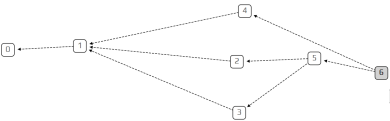
\includegraphics[width=3.0in]{screenshot001}
	\caption{DAG shows [1]}
	\label{simulationfigure}
\end{figure}

\subsection{Trading}
\subsubsection{Creation Trading}
There is no concept of mining in StreamNet, and all tokens are included in the creation transaction block. In Figure 2, a creation transaction is described with an initial token number of 5.

\begin{figure}[H]
	\centering
	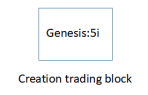
\includegraphics[width=2.0in]{screenshot002}
	\caption{Genesis Block}
	\label{simulationfigure}
\end{figure}

\subsubsection{Trading Content}
Assume that in Figure 2, Genesis wants to transfer 1 token to Alice, and then hopes to transfer 1 token to Bob and attach the transaction block corresponding to this transfer to StreamNet, then the resulting StreamNet is shown in Figure 3. Here, each transaction must find two tip transactions to confirm, namely trunk and branch transactions. For example, Genesis $\rightarrow$ Alice's transaction confirms the Genesis transaction itself, while Genesis $\rightarrow$ Bob's transaction confirms the Genesis transaction itself and Genesis $\rightarrow$ Alice's transaction. When a transaction wants to be attached to StreamNet, it must do enough Workload Proof (POW) [2], but this POW differs from Bitcoin in that its difficulty is fixed and therefore does not need to be The participation of miners [3].

\begin{figure}[H]
	\centering
	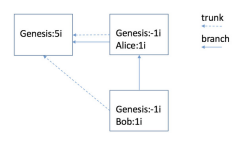
\includegraphics[width=3.0in]{screenshot003}
	\caption{shows the transfer transaction}
	\label{simulationfigure}
\end{figure}

\subsubsection{transaction verification (approve)}
Because a new transaction needs to find two tip transactions for approval, the verification method has two steps:
\begin{itemize}
\item with Genesis, verify all transactions that are directly or indirectly referenced, mainly to see if this will result in a negative balance or loss of the token [1]. For example, in Figure 4, Alice $\rightarrow$ Sam's transfer needs to verify transactions that are indirectly or directly referenced. Then it constructs a topological sequence according to the characteristics of DAG, namely (Genesis) $\rightarrow$ (Genesis $\rightarrow$ Alice) $\rightarrow$ (Genesis $\rightarrow$ Bob) $\rightarrow$ (Alice $\rightarrow$ Sam), and finds that each step does not violate the principle of transfer. Then the verification is successful. In Figure 5, the same topology sequence, when verifying (Genesis $\rightarrow$ Bob), because the Genesis balance will be reduced to -1, the verification fails, as an honest node, Alice $\rightarrow$ Sam transaction Will find a new tip to verify, but it can also choose to spoof, attach this transaction to the selected tip. However, such an approach is likely to result in subsequent rejection of its own transactions.
\item At the same time, the signature needs to be checked during the verification of the topology sequence to ensure that the link relationship has not been tampered with.
\end{itemize}

\begin{figure}[H]
	\centering
	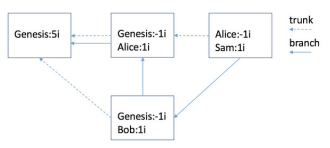
\includegraphics[width=3.0in]{screenshot004}
	\caption{confirms successful transaction}
	\label{simulationfigure}
\end{figure}

\begin{figure}[H]
	\centering
	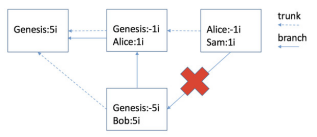
\includegraphics[width=3.0in]{screenshot005}
	\caption{confirms the failed transaction, which will cause the Genesis balance to drop to -1}
	\label{simulationfigure}
\end{figure}

\subsubsection{Select tip}
There are two basic concepts in StreamNet, one is the transaction rate, which indicates the number of transactions per time unit. For convenience, we set the time unit to seconds. The other is invisible time, indicating how many time units a transaction has not been seen by other exchanges after attach. Because of some existence, the transaction rate has an important influence on the shape of StreamNet. For example, in Figure 7, when the transaction rate is slow, StreamNet is more like a chain. In the case of block trading in Figure 8, the shape of StreamNet is a star.

\begin{figure}[H]
	\centering
	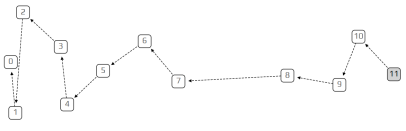
\includegraphics[width=3.0in]{screenshot006}
	\caption{StreamNet shape under slow trading}
	\label{simulationfigure}
\end{figure}

\begin{figure}[H]
	\centering
	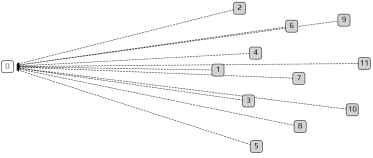
\includegraphics[width=3.0in]{screenshot007}
	\caption{StreamNet shape under fast trade}
	\label{simulationfigure}
\end{figure}

One of the most basic tip selection algorithms is to start from Genesis to move the transaction with approval to an equal probability until a tip is selected, as shown in Figure 8. Suppose Alice $\rightarrow$ Sam's transaction wants to select tip, which starts from Genesis transaction. There are two options for this time, one is Genesis $\rightarrow$ Alice, the other is Genesis $\rightarrow$ Bob, the probability of selecting Genesis $\rightarrow$ Alice is 1 /2, while Genesis $\rightarrow$ Bob is 1/2. 

\begin{figure}[H]
	\centering
	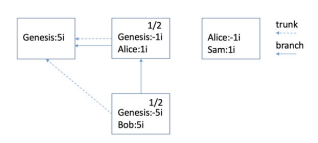
\includegraphics[width=3.0in]{screenshot008}
	\caption{Equal Probability Random Walk Algorithm}
	\label{simulationfigure}
\end{figure}

\begin{figure}[H]
	\centering
	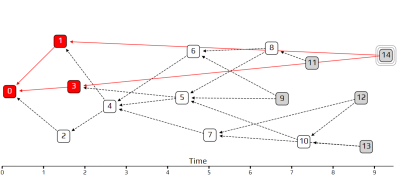
\includegraphics[width=3.0in]{screenshot009}
	\caption{lazy transaction example}
	\label{simulationfigure}
\end{figure}

\begin{figure}[H]
	\centering
	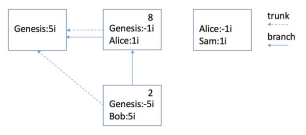
\includegraphics[width=3.0in]{screenshot010}
	\caption{Random walk selection tip}
	\label{simulationfigure}
\end{figure}

\begin{figure}[H]
	\centering
	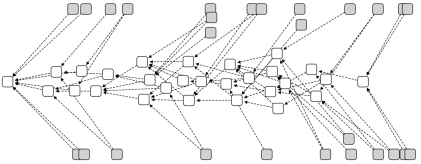
\includegraphics[width=3.0in]{screenshot011}
	\caption{super-weight algorithm example diagram}
	\label{simulationfigure}
\end{figure}

The problem with the basic random walk algorithm is that it produces lazy transactions. For example, in Figure 9,transaction 14 is a lazy transaction that causes new transactions to approve older transactions without being penalized. This problem can be solved by using Monte Carlo Random Walk (MCMC). In Figure 10, there is a weight on both transactions, for example, Genesis $\rightarrow$ Alice is 8, and Genesis $\rightarrow$ Bob is 2, then the probability of selecting Genesis $\rightarrow$ Alice is 8/10, and Genesis $\rightarrow$ Bob is 2 /10. The determination of the weight is determined by how many transactions have directly or indirectly approved the transaction. The more approved transactions, the greater the weight. If only deterministic use weights are then a super-weight algorithm, meaning that large-weight transactions are always preferred. The problem with this algorithm is that there are many transactions that can never be confirmed. Figure 11 shows the results of a super-weighted algorithm. For example, if purely using probability weighting, then it is a
super-probability algorithm. The trade-off between the two is represented by a $\alpha$, and it can be considered that the
larger the $\alpha$ is, the smaller the randomness is. The method of specifically using $\alpha$ to calculate the jump probability is expressed in the formula (1). Which represents the weight of the trading node.Where P\_{xy} represents the probability of jumping from x to y. H\_{y} represents the weight of the trading node y.

\begin{equation}
\label{simple_equation}
P_{xy} = \frac{e^{\alpha H_{y}}}{\Sigma_{z:z \rightarrow x}e^{\alpha H_{z}}}
\end{equation}

\subsubsection{Trading Consensus}
There are currently three ways to confirm a transaction in StreamNet:
	\begin{itemize}
		\item The first way is that the common nodes covered by all the previous tips are considered to be fully confirmed; for example, in Figure 12, the nodes referenced or indirectly referenced by tip1 are blue and yellow line covered transactions, while the tip2 reference Or the indirectly referenced node is a yellow line covered transaction. If there are only 1, 2 tips in StreamNet, then the green node is a fully confirmed transaction, while the green node is an unconfirmed transaction.
		\item The second way is that the system sends a Coordinator tip every 1 minute. This tip is called milestone and is attached to StreamNet. All transactions referenced by this Coordinator tip are confirmed.
		\item The third way is to use Monte Carlo Random Walk (MCMC). Call N times to select a tip using the tip selection algorithm. If a trading node is referenced by this tip, its credibility is increased by 1. After M selections have been cited M times, then the credibility is M / N.
  \end{itemize}

\begin{figure}[H]
	\centering
	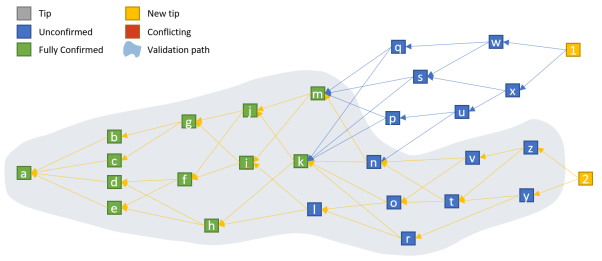
\includegraphics[width=3.0in]{screenshot012}
	\caption{fully confirms the node, unconfirmed node [4]}
	\label{simulationfigure}
\end{figure}

\section{Problems with existing DAGs}
\subsection{Network synchronization}
When a node accepts a request to attach a transaction and attaches the transaction to the local StreamNet, it broadcasts the changes made to its own neighboring machine. When the neighboring machine receives the update, it will follow the basic principles of attaching StreamNet. This update is attached to its own StreamNet and this update is further broadcast. If this update cannot be accepted by a large number of neighboring machines, the probability of being accepted by the entire network is greatly reduced. There are several problems in this:
\begin{itemize}
	\item Issues with offline updates. Offline updates are recognized in StreamNet, but when they are re-online, it will broadcast all local updates, but their local updates will only be accepted in the entire network and will not be partially accepted [4].
	\item How to recognize that a locally confirmed transaction is a transaction accepted by the whole network. How to express it on the wallet is a relatively big problem. In Bitcoin, there is no honest chain and dishonest chain. It is mainly realized by the cost of lying, that is, the POW of exponential growth, wanting to revert the transaction, or constructing the wrong chain. The price is very high. For a wallet, the time to verify a chain is the complexity of polynomial. In this way, we must believe that the data of a certain node in the whole network can be done. Although there are POWs in the current DAG, the complexity of constructing StreamNet itself is polynomial, so for the lying node, it can use a large computing power to construct a wrong StreamNet to mislead the transaction wallet.
	\item Existing DAGs are currently unable to guarantee strong consistency in the network environment [5].
\end{itemize}

\begin{figure}[H]
	\centering
	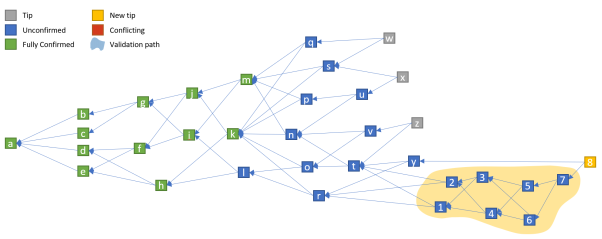
\includegraphics[width=3.0in]{screenshot013}
	\caption{Example of offline update [4]}
	\label{simulationfigure}
\end{figure}

\begin{figure}[H]
	\centering
	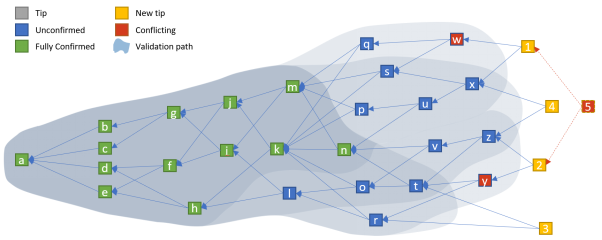
\includegraphics[width=3.0in]{screenshot014}
	\caption{Example of double flower problem}
	\label{simulationfigure}
\end{figure}

\subsection{double flower problem}
The double flower problem refers to the problem that the same token is used multiple times, which can be represented by the example in Figure 9, where the two transactions of w and y are double flower transactions, and the transaction 5 is the one that finds that this is a double flower transaction. Transaction. In the transaction consensus, it is obviously impossible to use the 100\% tip confirmation, because there will always be new transactions coming in to break the 100\% confirmation fact. This is called propagation delay [4]. If a random walk algorithm is used, given a confidence level (say 95\%), one of the transactions will naturally receive more transaction approvals in the natural state (without being subjected to a power attack), thus giving it confidence. The degree reaches a state sufficient to be confirmed. For example, as shown in Figure 10, w receives more confirmations in the future, and slowly y is isolated to lose the possibility of being confirmed. But when the fraudster's power is strong enough, it can issue enough transactions to approve w after a transaction is confirmed, then in this case, the previously confirmed transaction will in turn be marginalized. To achieve the purpose of double-flowering, such an attack is a replay attack, and it is necessary to accumulate 34\% of the computing power of the whole network to achieve the goal [6]. However, considering the low number of transactions in the entire network in the early stage [7], 34\% of the power attack is actually not difficult. In order to solve such problems, the transaction confirmed by the coordinator is absolutely valid, so regardless of the computing power of the follow-on attacker. Powerful, can not beat the coordinator's one-vote veto [1]. \\ 
\indent Therefore, the double flower problem is essentially a computing power problem, and it is also the essential problem of the existing DAG system. The introduction of the coordinator is a centralized solution, and in the future, as more and more devices join the StreamNet network, the role of the coordinator It will become unnecessary, and how to remove it to turn DAG into a decentralized network is a challenge [8].

\begin{figure}[H]
	\centering
	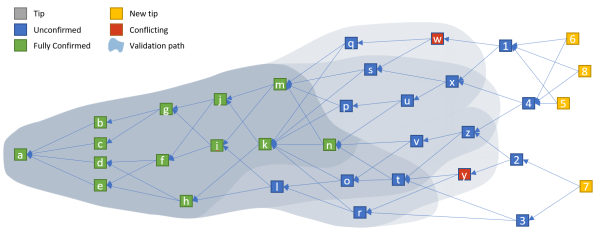
\includegraphics[width=3.0in]{screenshot015}
	\caption{Randomly solve the problem of double-flowering}
	\label{simulationfigure}
\end{figure}

\subsection{transaction confirmation speed problem}

\begin{figure}[H]
	\centering
	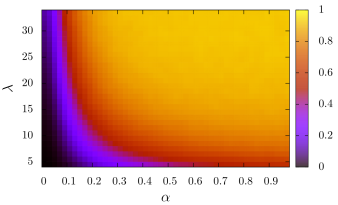
\includegraphics[width=3.0in]{screenshot016}
	\caption{The probability of a transaction being permanently stuck (failed), which is random, is the transaction rate [9]}
	\label{simulationfigure}
\end{figure}

The speed at which the transaction is confirmed and the likelihood that the transaction will be finalized depends on two factors, the first is the transaction rate $\lambda$, and the second is the randomness $\alpha$. From Figure 16, it can be seen that the probability of increasing the success of the transaction is mainly to increase the transaction. The rate reduces randomness, and in Figure 17, a more intuitive expression of the effect of $\alpha$ can be seen, under the same conditions, the higher the unconfirmed transaction becomes more. However, because the transaction rate in the whole network is relatively slow, there are not many active nodes, and some optimization methods have been proposed. For example, the method of coordinator mentioned above and the method of Reattach, rebroadcast [10], etc. It can be attributed to the method of human intervention.

\subsection{Encryption Algorithm Vulnerabilities}
Because the current DAG encryption algorithm is based on Trytes, and the encryption algorithm is invented by itself, the method pointed out in [11] can find the hash collision in a few minutes using ordinary computers. The attacker can use this vulnerability to fake other users. Signature, fundamentally disintegrating the security of IOTA.

\subsection{ replay attack}
Replay attacks In addition to the use of power to attack in the double-flower problem, two attack modes are mentioned in the white paper, the first one is a side chain attack and the other is a double-sided chain attack [12]. 

\begin{figure}[H]
	\centering
	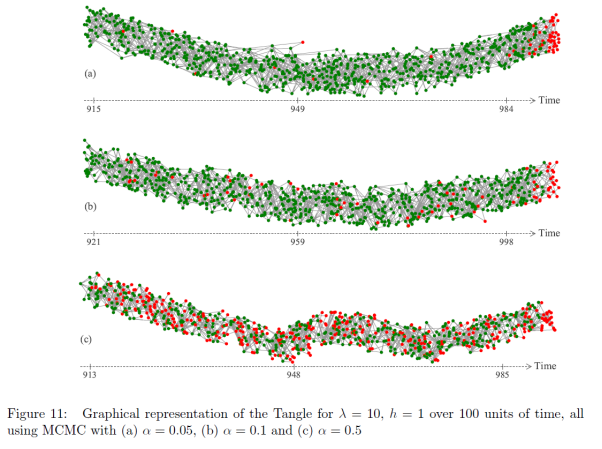
\includegraphics[width=3.0in]{screenshot017}
	\caption{a more intuitive expression of the role}
	\label{simulationfigure}
\end{figure}

\section{StreamNet main algorithm}
\subsection{Based on the centrality (katz centrality) to COO starting point selection algorithm}
At this stage of the DAG, when selecting the tip, it will not start from the creation transaction, but will simply start with a coordinator as the starting point. This will lead to a centralization problem. So the first question we considered when designing StreamNet was how to remove the COO and achieve a truly distributed DAG. So we need a consensus authoritative transaction as a starting point rather than a coordinator mandated by a centralized node as a starting point. Here we choose katz centrality [13] as the starting point for selection criteria. In StreamNet, we use an Adjacency Matrix to represent the link relationship between transactions, which is used to represent, and a second-order link matrix (representing the number of nodes that jump from node to node by two steps). Similarly, we represent k-order link matrix. . Then the importance vector of each node can be calculated by (2). Where is an importance weight vector, which is a matrix of all ones. Because the transactions in StreamNet are constantly entering the network, if you need to recalculate the Katz center degree every time you make a tip selection, then the complexity will be very large, so you need a streaming computing framework. To dynamically update the Katz center degree based on the newly added nodes, we use an incremental algorithm to deal with the flow graph calculation [14].

\begin{equation}
\label{simple_equation}
\sum_{k=1}^{max} \alpha^{k-1}A^{k}=A(I-\alpha A)^{-1}
\end{equation}

It should be noted that in the calculation results, we do not need to find the most transactions in the center of Katz, because this transaction is always a Genesis transaction, so we should find this in the recent transaction between Katz centrality and time. Initial node.

\subsection{Considering the transaction weight algorithm of edge information}
Because the attacker can attack the main network (Main StreamNet) in different forms, a typical scenario in which we consider the double-flower problem is the Simple Parasite Chain attack. A simple side chain is shown in Figure 18. In [15], the initiator proposed to use local modifier to solve the attack, but since there is no relevant code, we will not discuss it here. Here we discuss our weight update algorithm with side information. The framework of this algorithm is consistent with the framework of the weight update algorithm in the existing DAG. The difference is that when making a set join between two approve transactions, a weighted set join is performed, and the weight is determined. It is determined by the information of the side, and the information of the side is mainly confirmed by time. For example, in Figure 1, assume that each edge is given a weight w1-w12 transaction 5 because it is approved by transactions 6, 7, 8 and its weight information is [5,7*(w1*w6+*w2) , 8*w3, 6*w6]. \\
\indent The reason for the side information is that the attacker often sends out a large number of transactions within a short period of time and approves each other to achieve the purpose of rapidly growing the side chain. And because the edge information is used to rescale the transaction, the trading effects of these attacks are attenuated. On the contrary, the non-attack type transaction is similar to the speed of the whole network, and its weight update is similar to the result of the original algorithm.

\begin{figure}[H]
	\centering
	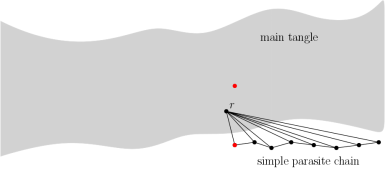
\includegraphics[width=3.0in]{screenshot018}
	\caption{simple sidechain attack [16], a series of deceptive sidechains will refer to a transaction r in the main network, when the SPC grows to a certain extent, it may lead to double success, the two in the figure A red dot represents a double flower transaction}
	\label{simulationfigure}
\end{figure}

\begin{figure}[H]
	\centering
	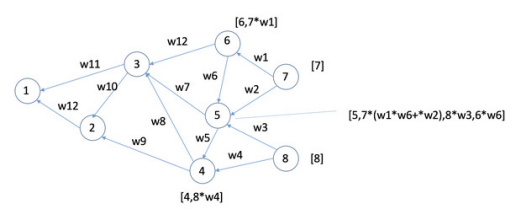
\includegraphics[width=3.0in]{screenshot019}
	\caption{Example of trading weights with side information}
	\label{simulationfigure}
\end{figure}

    %\begin{algorithm}[H]
	%\caption{Algorithm for calculating cumulative weight}
	%\KwIn{G^{'}=(V^{'} , E^{'})}
	%\KwOut{Cumulative weight}
	%graph traversal (BFS $\mid$ DFS) \Rightarrow  F(s) \; \\
	%V \gets F(s)\; \\
	%G(V,E) \Rightarrow G[F(s)]\,\,(\,let\,G(V,E)\,be\,the\,induced\,subgraph\,G[F(s)])\;   \\
	%Initialize\,F(v) \Leftarrow \left\{ \right\} for\,all\,v\in V\; \\
	%SortedVertices \Leftarrow topological\,sorting\,of\,G\; \\
	%\ForAll {$v$ such that $v\in SortedVertices$}{   
	%	\For{$i=v$ to $u$}{   
	%		\ $F(u) \Leftarrow $ F(u) + (F(v) + \left\{v\right\}) \ast w \; 
	%		}
	%	CumulativeWeight[v] \Leftarrow \left|F(v)\right| \; \\
	%	(Optimization)\,Free\,the\,memory\,taken,by\,F(v), as\,it\,no\,longer\,used
	%}	
	%\end{algorithm}

\subsection{Weight update algorithm based on flow graph calculation}
When updating the weight, the static graph algorithm needs to calculate the weight of each node from the beginning of the initial recognition node. The complexity of this algorithm is , if our static calculation information is cached, when the new tip is added. By updating the already cached information, the complexity of calculating the weight each time the tip is added can be differentiated . But there is also a problem with this, the spatial complexity of this algorithm will become . How to design a streaming algorithm to reduce the complexity of time space complexity to  is a challenge.

\begin{figure}[H]
	\centering
	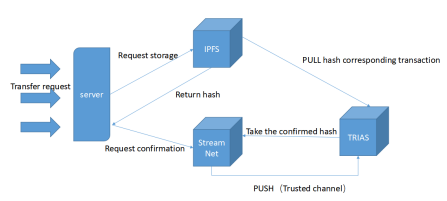
\includegraphics[width=3.0in]{screenshot020}
	\caption{StreamNet shows the TRIAS transfer request cache}
	\label{simulationfigure}
\end{figure}

\subsection{Using StreamNet in conjunction with IPFS to cache TRIAS transfer requests}
StreamNet can be used to cache and pre-confirm other low-traffic blockchain systems because of its high throughput. TRIAS as a cross-blockchain system can take advantage of this feature to achieve its high degree of expansion, which can achieve the ability of elastic The specific structure is shown in Figure 20. There is a distributed transfer service. When an external transfer request comes over, it first stores the information transferred from the IPFS and gets a hash. The transfer server then constructs a hashNet transaction. When the traffic is small, StreamNet can directly push the hash of the transaction to TRIAS after confirming the transaction hash, so TRIAS can get the specific transfer information from IPFS and package the transfer. When the traffic is large, StreamNet will continue to confirm These transactions. When TRIA is idle, it will pull the confirmed hash to StreamNet, and get the specific transfer information from IPFS and package the transfer.

\section{Bibliography}
\begin{thebibliography}{ } 
	\bibitem{latexcompanion}
	\textit{A.Gal,"The\,Tangle:an\,Illustrated\,Introduction,"[Online].Available: https://blog.iota.org/the-tangle-an-illustrated-introduction-4d5eae6fe8d4.}
	\bibitem{latexcompanion}
	\textit{I.o.doc,"PoW\,on\,the\,Tangle,"[Online].\,Available: https://docs.iota.org/introduction/tangle/proof-of-work.}	
	\bibitem{latexcompanion}
	\textit{M.Wind,"Everything you didn’t know about IOTA,"[Online].Available: https://medium.com/@mistywind/iota-fud-answered-by-a-non-techie-enthusiast-2312325fddb6.}
	\bibitem{latexcompanion}
	\textit{noneymous,"iota-consensus-presentation,"[Online].Available: https://github.com/noneymous/iota-consensus-presentation.}
	\bibitem{latexcompanion}
	\textit{Wang\,Tao,"Technology\,veterans\,vomiting\,blood\,sharing:about\,the\,advantages\,and disadvantages\,of\,the\,consensus\,mechanism\,of\,blockchain,"[Online].Available: http://www.huoxing24.com/newsdetail/2018032521054168745.html.}
	\bibitem{latexcompanion}
	\textit{Xdag\,Communicate\,the\,community,"10\,minutes\,to\,understand\,the\,transition\,technology of\,blockchain——DAG,"[Online].Available: https://www.jinse.com/bitcoin/254086.html.}
	\bibitem{latexcompanion}
	\textit{Fire\,Coin\,Network,"[Beyond\,White\,Paper\,3]DAG\,Technology\,Analysis\,and\,Measurement," [Online].Available: https://www.jinse.com/bitcoin/212928.html.}
	\bibitem{latexcompanion}
	\textit{X.Qian,"IOTA\,Introduction\,and\,Improvements,"[Online].Available: https://zhuanlan.zhihu.com/p/33009843.}
	\bibitem{latexcompanion}
	\textit{A.Gal,"Confirmation\,rates\,in\,the\,Tangle,"[Online].Available: https://blog.iota.org/confirmation-rates-in-the-tangle-186ef02878bb.}
	\bibitem{latexcompanion}
	\textit{J.Hu,"IOTA Tangle:Introductory overview of white paper for Beginners,"[Online].Available: https://hackernoon.com/iota-tangle-introductory-overview-of-white-paper-for-beginners-df9b14882b64.}
	\bibitem{latexcompanion}
	\textit{N.Narula,"Cryptographic\,vulnerabilities\,in\,IOTA,"[Online].Available: Cryptographic vulnerabilities in IOTA.}
	\bibitem{latexcompanion}
	\textit{S.Popov,"On the Tangle, White Papers, Proofs, Airplanes, and Local Modifiers,"[Online].Available: https://blog.iota.org/on-the-tangle-white-papers-proofs-airplanes-and-local-modifiers-44683aff8fea.}
	\bibitem{latexcompanion}
	\textit{l.katz,"A NEW STATUS INDEX DERIVED FROM SOCIOMETRIC ANALYSIS,"psychometrika,no.1,3\,1953.}
	\bibitem{latexcompanion}
	\textit{D.B.Eisha Nathan,"Incrementally updating Katz centrality in dynamic graphs," Social Network Analysis and Mining, 2018. }
	\bibitem{latexcompanion}
	\textit{S.Popov,"On the Tangle, White Papers, Proofs, Airplanes, and Local Modifiers,"[Online].Available: https://blog.iota.org/on-the-tangle-white-papers-proofs-airplanes-and-local-modifiers-44683aff8fea.}
	\bibitem{latexcompanion}
	\textit{B.Kuśmierz,"Attack\,analysis\,-\,the\,simple\,parasite\,chain,"[Online].Available: https://blog.iota.org/attack-analysis-the-simple-parasite-chain-42a34bfeaf23.}
	\bibitem{latexcompanion}
	\textit{R.Y.J.L.William\,L.Hamilton,"Representation Learning on Graphs: Methods and Applications," arXiv:1709.05584, 2017.}
	\bibitem{latexcompanion}
	\textit{S.Popov,"The Tangle V 1.4.3," N/A, 2018.}
	\bibitem{latexcompanion}
	\textit{B.K.P.S.A.Gal,"Extracting Tangle Properties in Continuous Time via Large-Scale Simulations," IOTA Foundation, 2018.}
	\bibitem{latexcompanion}
	\textit{J.Cech,"IRI 1.5.0 — New\,tip\,selection\,algorithm\,and\,other\,improvements,"[Online].Available: https://blog.iota.org/new-tip-selection-algorithm-in-iri-1-5-0-61294c1df6f1.}
	\bibitem{latexcompanion}
	\textit{I.foundation,"IOTA\,Tangle\,visualization,"[Online].Available: https://public-qnbiiqwyqj.now.sh.}
	\bibitem{latexcompanion}
	\textit{Ms.Miss\,City,"Can\,a\,directed\,Acyclic\,DAG\,become\,an\,IoT\,backbone\,network?\,IOTA\,accelerates\,application\,landing,"[Online].Available: https://zhuanlan.zhihu.com/p/39928206.}
	\bibitem{latexcompanion}
	\textit{A.Gal,"Alpha:playing\,with\,randomness,"[Online].Available: https://blog.iota.org/alpha-d176d7601f1c.}
	\bibitem{latexcompanion}
	\textit{C.Shikhelman,"Validity\,in\,the\,Tangle:The\,good,\,the\,bad,\,and\,the\,ugly,"[Online].Available: https://blog.iota.org/validity-in-the-tangle-the-good-the-bad-and-the-ugly-98bd3b53408a.}
\end{thebibliography}

\section{Briefly introduce our overall work}
\begin{itemize}
	\item Incentive:
		\begin{itemize}
			\item Use IOTA as a building block for their TRIAS blockchain
			\item Improving IOTA, make it faster and more robust and Coo-free
		\end{itemize}
	\item How do we do it: 
	\begin{itemize}
		\item TRIAS's own Intelligence Property, cannot share too many details (not meant for IoT)
		\item TRIAS’s code will be compatible with the IOTA protocol, while it will serve its own purpose
		\item May eventually send PR / share TRIAS’s code
	\end{itemize}
\end{itemize}

\section{Technical details discussion}
\begin{itemize}
	\item oo-free related:
	\begin{itemize}
		\item Katz Centrality Can be used for Entry point selection
		\item IOTA foundation have done some work in mapping it out, they can share, can ping gal.rogozinski@iota.org to ask for a map of Coo-dependencies in IRI
		\item “Dangling tx problem”: transactions get left behind if they don’t get approved early
		\item Detecting side tangle attacks: cannot share specifics, need to get an OK from bosses
	\end{itemize}
	\item Attack related: 
	\begin{itemize}
		\item Katz Centrality Can be used to detect attacks (by identifying community structures)
		\item we can let people tag attacker txs and train an algorithm to identify patterns. Basic idea is like GAN
		\item Edge weights are used to detect attackers. The idea is that attackers will probably release “dense” transactions. In other words, the time between attacker txs would be small (seems to be the opposite idea of LM). Doesn’t work so well so will probably be left out. It works pretty well for small lambda. It’s the approvee that gets punished if it has lots of approvers with small time differences. However, this could allow censoring transactions
		\item And all above methods are obeying the local modifier ide
	\end{itemize}
	\item Transaction speed related (tip selection):
	\begin{itemize}
		\item Streaming algorithms can be used to avoid computation from scratch
		\item Katz Centrality Meant to be used in tip selection as well (instead of MCMC?)
		\item Also considering using ML to analyze the graph (nothing done yet)
	\end{itemize}
		\item Transaction confidence:
	\begin{itemize}
		\item Katz Centrality can be used for computing confidence (knowing whether a tx is confirmed)
	\end{itemize}
		\item Economic Analysis:
	\begin{itemize}
		\item oanalyzing communities, aside from avoiding attacks? Currently no specific role, but maybe economic analysis in the future.C
	\end{itemize}
\end{itemize}

\section{Cover at the end}
\begin{itemize}
	\item Considerations for alpha:
	\begin{itemize}
		\item https://blog.iota.org/confirmation-rates-in-the-tangle-186ef02878bb
	\end{itemize}
\end{itemize}
\begin{itemize}
	\item Why we choose to accept some \% of left-behind txs
	\begin{itemize}
		\item We want eventual finality: a high certainty that after some given time, a tx has either confidence 0 or 1
		\item oDirect connection between small alpha and high confirmation rate (low \% of txs left behind)
	\end{itemize}
\end{itemize}
\begin{itemize}
	\item My issues with Katz centrality
	\begin{itemize}
		\item Not proportional to PoW
		\item Puts stronger emphasis on Tangle topology (vs cumulative weight)
	\end{itemize}
\end{itemize}
\begin{itemize}
	\item Our version of “streaming CW”
	\begin{itemize}
		\item Lazy in IRI, optimal for low-usage nodes
		\item Caching tips (selecting 100 tip pairs, they expire after a few seconds)
		\item Weight propagation O(N) (eager). For each incoming transaction, you add 1 to the weights of all its past cone / referenced txs
		\item Set-union algorithm has same asymptotic complexity as naive DFS for CW computation (still can be optimized, will share soon)
		\item ZY: has some doubts about the correctness
	\end{itemize}
\end{itemize}
\begin{itemize}
	\item Timestamps
	\begin{itemize}
		\item Some tx timestamps are signed (cryptographically), and some are not
		\item There is no order enforced and they may contain arbitrary data
		\item Find link for tx anatomy fields description
		\item Only reliable timestamp is receivedTime (pretty sure about the name), which is subjective to the node. This is the time you first received this tx
	\end{itemize}
\end{itemize}
\begin{itemize}
	\item My issue with ML
	\begin{itemize}
		\item AG is concerned with using ML to define core consensus algorithm (includes tip selection), because it may be gameable
	\end{itemize}
\end{itemize}

\begin{itemize}
	\item Description of our methodology for “parasite chain” attack analysis
	\begin{itemize}
		\item Exactly the same as “side chain” from the whitepaper
		\item We’re starting by examining the simplest shape we can think of
		\item oBlog post about it:
		\begin{itemize}
			\item https://blog.iota.org/confirmation-rates-in-the-tangle-186ef02878bb
		\end{itemize}
	\end{itemize}
\end{itemize}

\end{document}








































